\chapter{Теоретическое исследование}
\section{Предлагаемая схема параллелизации}
Рассмотрим две основные процедуры в алгоритме Фортена с модификацией Буздалова --- \textsc{NDHelperA} и \textsc{NDHelperB}.
Обе процедуры являются рекурсивными и следуют принципу <<разделяй и властвуй>>.
Входящие множества точек разделяются на три части $L$, $M$, $H$ относительно медианного значения по $k$-й координате.
Далее \textsc{NDHelperA} и \textsc{NDHelperB}, используя тот факт, что точки из подмножества $H$ не могут доминировать точки из $M$, а точки из $M$ не могут доминировать точки из $L$, рекурсивно запускают подзадачи с уменьшением размерности $k$.
Деление задач происходит до того момента, когда размерность $k$ станет равна $2$, что в дальнейшем обрабатывается процедурами \textsc{SweepA} и \textsc{SweepB} соответственно.

\subsection{NDHelperB}
Можно заметить, что на момент вызова процедуры \textsc{NDHelperB(L, H, k)} ранги точек из множества $L$ уже вычислены и в дальнейшем остаются неизменными.
Также заметим, что для корректной работы процедуры, каждая точка из множества $H$ должна быть сравнена с каждой точкой из множество $L$, но при этом порядок сравнений не влияет на результат.

Таким образом мы можем заключить, что рекурсивные вызовы подзадач в теле \textsc{NDHelperB} являются независимыми и порядок их исполнения не влияет на корректность алгоритма.
Более того, мы можем разделить множество $L$ на любое количество частей ${L_1, L_2,\ldots, L_n}$ и тогда результат исполнения \textsc{NDHelperB($L_i$, H, k)} для всех $1\leq i\leq n$ будет идентичен результату исполнения \textsc{NDHelperB(L, H, k)}.
Следовательно, \textsc{NDHelperB} допускает возможность параллельного исполнения.

\begin{figure}[h]
\centering
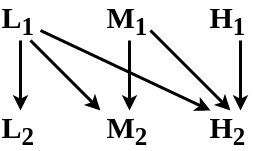
\includegraphics[width=0.4\textwidth]{images/ndb.png}
\caption{Вызовы подзадач в \textsc{NDHelperB}}
\end{figure}

\subsection{NDHelperA}
\subsubsection{Асинхронное исполнение}
С параллелизацией процедуры \textsc{NDHelperA} возникают определенные сложности.
Внутренние вызовы \textsc{NDHelperA} и \textsc{NDHelperB} зависят друг от друга и имеют строго определенную последовательность. 
Например, перед выполнением \textsc{NDHelperA(M, k-1)} вычисления в процедурах \textsc{NDHelperA(L, k)} и \textsc{NDHelperB(L, M, k-1)} уже должны быть выполнены.

Тем не менее, опираясь на утверждение из предыдущей секции, мы можем заметить, что как только ранги какого-то левого подмножества входящих точек будут вычислены, мы сразу же можем начать сравнивать эти точки с подмножествами точек, лежащими правее по $k$-й координате, при помощи процедуры \textsc{NDHelperB}.

\begin{figure}[h]
\centering
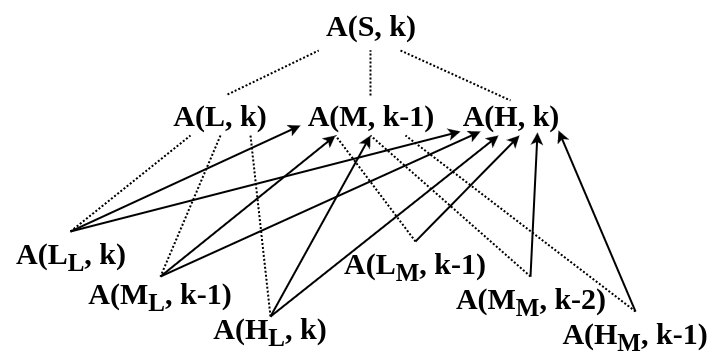
\includegraphics[width=\textwidth]{images/async.png}
\caption{Идея параллелизации процедуры \textsc{NDHelperA}}
\end{figure}

Пусть подмножество $L$ в вызове \textsc{NDHelperA(L, k)} посредством \textsc{SplitBy} поделится на три части по $k$-й координате: $L_L$, $M_L$ и $H_L$.
Заметим, что вместо \textsc{NDHelperB(L, M, k-1)} мы можем асинхронно вызывать \textsc{NDHelperB(Ll, M, k-1)}, \textsc{NDHelperB(Ml, M, k-1)}, \textsc{NDHelperB(Hl, M, k-1)} по мере вычисления рангов каждой из частей.

Точно таким же образом мы можем начать сравнивать точки из $L_L$, $M_L$, $H_L$ и $L_M, M_M, H_M$ с точками из $H$ как только ранги этих точек уже будут известны.
Эту идею можно развить дальше, разделив вызовы \textsc{NDHelperB} на более мелкие подзадачи.

\subsubsection{Плюсы и минусы модификации}
Основная задача, которая решается асинхронным выполнением подзадач \textsc{NDHelperB} в \textsc{NDHelperA} --- минимизация бездействующих потоков исполнения.
Однако выигрыш от модификации процедуры \textsc{NDHelperA}, описанной выше, будет заметен только при достаточном количестве процессоров.

Заметим, что \textsc{NDHelperB(L, H, k)} и \textsc{SweepB(L, H)} используют инвариант лексикографического порядка во входных списках точек, что позволяет проходить оба подмножества ровно один раз, используя два указателя.
Если же мы поделим левое подмножество на $n$ частей и вызовем процедуру \textsc{NDHelperB} на каждой из них, то получится, что по правому подмножеству $H$ мы пройдем $n$ раз вместо одного. Таким образом, мы улучшаем степень параллельности алгоритма ценой увеличения объема дополнительной работы.

\subsubsection{Теоретическое доказательство эффективности}
Пусть у нас есть $O(N)$ процессоров. Сравним время работы последовательной и асинхронной версий.
Входное множество $S$ поделено на части $L$, $M$, $H$. Множество $L$ в свою очередь поделено на $L_L$, $M_L$, $H_L$ (см. рисунок 3).

Сравним время работы алгоритмов до начала исполнения \textsc{NDHelperA(M, k-1)}.
Обозначим время исполнения \textsc{NDHelperA} на $L_L$, $M_L$, $H_L$ как $A_1$, $A_2$, $A_3$ соответственно.
Время работы \textsc{NDHelperB(Ll, Ml)} и \textsc{NDHelperB(Ml, Hl)} как $B_{1,2}$ и $B_{2,3}$.
Время работы синхронного вызова \textsc{NDHelperB(L, M, k-1)} --- $B$, а асинхронных вызовов на подмножествах --- $B_1$, $B_2$, $B_3$.

При последовательном исполнении:
\begin{center}
    $T_{seq} = A_1 + B_{1,2} + A_2 + B_{2,3} + A_3 + B$
\end{center}

При асинхронном исполнении:
\begin{center}
    $T_{async} = A_1 + max(B_1, B_{1,2} + A_2 + max(B_2, B_{2,3} + A_3 + B_3))$\\
\end{center}

Пусть $B_1 > B_{1,2} + A_2 + max(B_2, B_{2,3} + A_3 + B_3)$, тогда:
\begin{center}
    $T_{async} = A_1 + B_1 < T_{seq}$, т.к. $B_1 < B$
\end{center}

В обратном случае:
\begin{center}
    $T_{async} = A_1 + B_{1,2} + A_2 + max(B_2, B_{2,3} + A_3 + B_3)$
\end{center}

Остается два варианта:
\begin{center}
    $T_{async} = A_1 + B_{1,2} + A_2 + B_2 < T_{seq}$\\
    $T_{async} = A_1 + B_{1,2} + A_2 + B_{2,3} + A_3 + B_3 < T_{seq}$\\
    т.к. $B_2 < B$ и $B_3 < B$
\end{center}

Таким образом, общее время работы алгоритма до момента ожидания результатов асинхронных вызовов \textsc{NDHelperB} всегда будет меньше, чем в последовательной версии, т.к. в обоих случаях вызываются абсолютно идентичные синхронные методы, а время обработки подмножества точек всегда меньше времени обработки целого множества.

Необходимо отметить, что данное доказательство корректно только при достаточном количестве процессоров.
В обратном случае эффективность алгоритма может ухудшиться, т.к. обработка части подзадач будет происходить последовательно.

\section{Улучшение процедуры SweepB}
Процедура \textsc{SweepB(L, H)} обновляет ранги точек из $H$, сравнивая их с точками из $L$ по первым двум критериям.
Как уже упоминалось в описании алгоритма, оба множества $L$ и $H$ отсортированы лексикографически, что позволяет проходить каждый список ровно один раз слева направо, используя метод заметающей прямой.
Также не будем забывать, что ранги точек из $L$ уже известны и окончательны.

В процедуре поддерживается множество $T$, в котором хранятся <<представители>> встречаемых фронтов точек. Представителем фронта $i$ всегда является точка с рангом $i$ и наибольшим значением по второму критерию. 
Это может быть любое сбалансированное дерево со значением по второму критерию в качестве ключа и номером фронта в качестве значения.

Т.к. мы спускаемся по дереву каждый раз, когда обновляем представителя фронта при итерации по $L$ и каждый раз, когда делаем запрос по второму критерию при итерации по $H$, то общее время работы процедуры --- $O((|L|+|H|)\log{|L|})$.

Пусть $A_i$ --- представитель фронта $i$, $A_j$ --- представитель фронта $j$, и $i < j$.
Тогда по определению: $A_i[0] \leq A_j[0]$ и $A_i[1] \leq A_j[1]$.
Отсюда следует, что при обновлении представителя фронта структура дерева не меняется.
Мы можем воспользоваться этим условием и не спускаться каждый раз по дереву, если фронт текущей точки из $L$ уже встречался.

Введем вспомогательную структуру $P$, массив размера $N$.
В $P[i]$ будем хранить указатель на вершину дерева $T$, где лежит представитель фронта $i$.
Если фронт $i$ еще не встречался, то в $P[i]$ будет лежать нулевой указатель.

\begin{figure}[h]
\centering
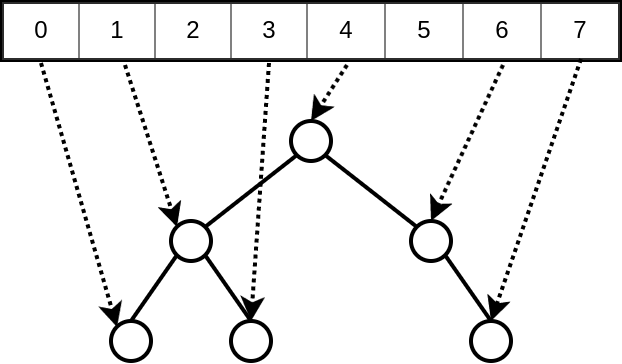
\includegraphics[width=0.7\textwidth]{images/sweep.png}
    \caption{Вспомогательный список указателей в \textsc{SweepB}}
\end{figure}

Таким образом, если ранг текущей точки --- $i$, и в дереве уже лежит какой-то представитель соответствующего фронта, то вместо cпуска по дереву за $O(\log(|L|))$ мы лишь изменим ключ вершины по ссылке $P[i]$ за $O(1)$.

В худшем случае, когда все точки из $L$ имеют различные ранги, время работы остается прежним.
Однако на практике чаще всего встречается ограниченное число рангов, поэтому описанная выше модификация существенно улучшит время работы \textsc{SweepB}.
